\documentclass[12pt,a4paper]{report}
\usepackage[utf8]{inputenc}
\usepackage[T1]{fontenc}
\usepackage{setspace}
\renewcommand{\baselinestretch}{1.7}
\usepackage[francais]{babel}
\usepackage[maxlevel=3]{csquotes}
\usepackage[backend=bibtex,style=verbose-trad1,isbn=false]{biblatex}
\DefineBibliographyStrings{french}{in={dans},inseries={dans}}
\usepackage[cyr]{aeguill}
\usepackage{geometry}
\geometry{verbose,letterpaper,tmargin=27.5mm,bmargin=27.5mm,lmargin=27.5mm,rmargin=27.5mm}
\usepackage{graphicx}
\usepackage[
    labelfont=sf,
    hypcap=false,
    format=hang,
    width=0.8\columnwidth
]{caption}
\usepackage{epigraph}
\setlength\epigraphwidth{13cm}
\usepackage{float}
\usepackage{url}
\usepackage{amsfonts}
%\newcommand{\guil}[1]{?~{#1}~?}    %guillemets
%\newcommand{\guill}[1]{``{#1}''}     %guillements dans les guillemets
\bibliography{bibliographie/bibliographiebdd}
\bibliographystyle{plain}

\begin{document}

\sloppy
\begin{titlepage}
  \begin{singlespace}
    \begin{center}
    {Université de Lille} \vspace{1.5 cm}\\
    \end{center}

    \begin{center}


      \Large{{\bf{Modèle de Potts pour la classification}}\\Master Mathématiques et Applications}


    \end{center}
    \vspace{1.5 cm}
    \begin{center}
      \normalsize{par Khalifa Naïl et Briouat Farid}
      \vspace{1.5 cm}
    \end{center}

    \begin{center}
      Département de Mathématiques\\
      Faculté des sciences et technologies
    \end{center}
    \vspace{1.5 cm}

    \begin{center}
      Mémoire présenté à la Faculté des sciences et technologies en vue de l'UE TER
    \end{center}
    \vspace{1.5 cm}






    \begin{center}
Mai 2023\\
\vspace{3 cm}
KHALIFA Naïl et BRIOUAT Farid
\end{center}
  \end{singlespace}

  \newpage
\end{titlepage} 
%\input{titres/garde.tex}



\begin{singlespace}
\tableofcontents % table des mati?res
\end{singlespace}

\pagenumbering{arabic}
\setcounter{page}{1}

\addcontentsline{toc}{chapter}{Remerciements}
\chapter*{Remerciements} 
Nous remercions Monsieur Nicolas Wicker pour son encadrement et son aide précieuse.
Nous remercions Madame Charlotte Baey notre enseignante de statistique computationnelle.




%dans les fichier vous trouverez des exemples d'usage des diff?rentes commandes de LaTeX

\addcontentsline{toc}{chapter}{Introduction}
\chapter*{Introduction}
\setcounter{chapter}{1}
\newcommand\tab[1][0.8cm]{\hspace*{#1}}

\begin{article}
    Étant étudiants en master Mathématiques et Application dans la section Ingénierie Statistique Numérique, l'étude d'évolution de cluster et de simulation grâce à des algorithmes MCMC\footnote{Markov chain Monte Carlo} nous semble assez logique.
Le but de notre TER est de réaliser une classification non supervisée d'un ensemble de point en utilisant le modèle de Potts.
On a donc procédé en deux étapes une premiere étape qui était l'implémentation d'un programme informatique en C++ et en Python.
Ces deux langages sont très utiles pour la modélisation qui se fera en Python et pour l'algorithmique qui se fera en C++.
Puis une deuxième partie qui est l'étude de l'algorithme de Metropolis-Hasting, sa convergence et l'utilité de cet algorithme dans un tel modèle.
Dans ce mémoire, nous allons ainsi expliquer en premier temps le travaille que nous avons fournis en programmation, ensuite nous allons, à l'aide de nos connaissances statistiques, l'utilité de l'algorithme de MH\footnote{Metropolis-Hasting}.
    \newline L'argumentation sera basée sur notre cours de statistique computationnel et de nos recherches référencées en fin de document.
    \newline \newline
    \tab Pour commencer, qu'est-ce que le modèle de Potts ?dsqsdq
    \newline D'après l'encyclopédie libre Wikipedia, le modèle cellulaire de Potts\footnote{CPM} est un modèle informatique de cellules et de tissus.
    Il est aussi connu sous le nom de modèle Glazier-Graner-Hogeweg.
    Le CPM est composé d'une grille rectangulaire où chaque pixel peut appartenir soit à une cellule, soit au milieu.
    Une cellule se compose donc d'un ensemble de pixels qui partagent le même état.
    L'algorithme qui met à jour les états de chaque pixel minimise cette énergie en suivant un algorithme de type MCMC.
    Ici nous utiliserons donc l'algorithme de Metropolis-Hasting.
    \newline \tab On suppose que l’on dispose de \textit{n} points $x_{1},...,x_{n}$
    \newline \[p_{T}(z)\propto\exp\Bigg\{-\frac{1}{T}\sum_{i=1}^{n}\sum_{j=1}^{n}(1-\delta_{ij})s(x_i,x_j)\Bigg\}\]

\end{article} %intro

%%! Author = nail
%! Date = 09/03/2023

% Preamble

\chapter{Programmation}
\setcounter{chapter}{1}

% Document
\begin{article}
    \section{Préambule}\label{sec:preambule}%
    Pour implementer le modèle de Potts, nous allons suivre le schema que nous avons mis en place afin de pouvoir générer des modèles le plus simplement possible.
    \newline On a donc diviser les taches selon ce schema :
    \newline
    \begin{figure}[ht]
        \centering
        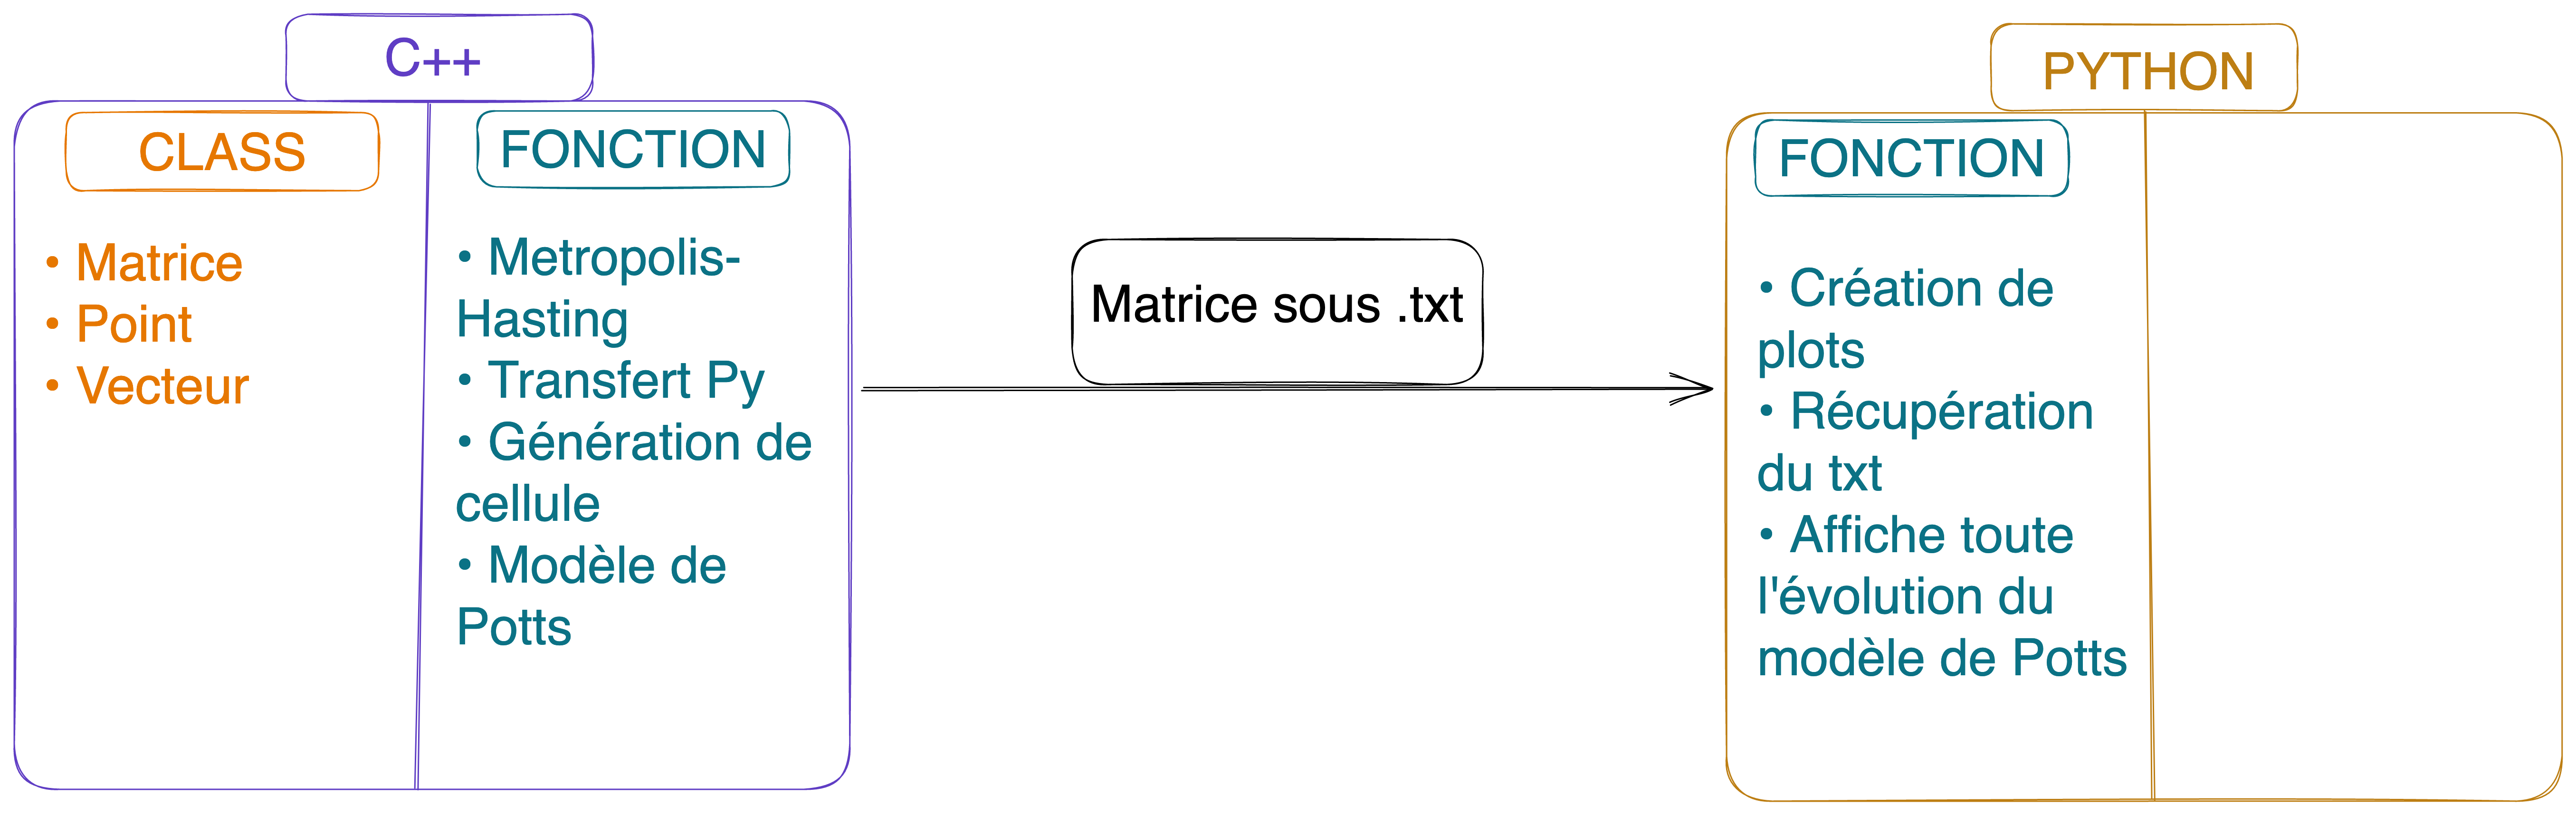
\includegraphics[scale=0.09]{./img/prog/Schema_prog}
        \caption{Schema de programmation}
        \label{fig:prog1}
    \end{figure}

    On a, selon ce schema, deux langages de programmation différents le C++ et le Python.

    \section{Explication}\label{sec:explication}
    \subsection{Préambul en C++}\label{subsec:preambul-en-c++}
    \noindent On va donc implémenter 3 classes différentes :
    \begin{description}
        \item[point] Une classe de point avec 2 coordonnées dont chacun ont un état, dans cette classe nous aurons des fonctions qui modifieront les propriétes des points.
        \item[matrice] Cette classe va nous permettre d'avoir une matrice de point.
        \item[vecteur-template] Ce n'est pas vraiment une classe, car ici nous allons utiliser la classe deja présente en C++, vector\footnote{Documentation officielle de la classe sur : https://cplusplus.com/reference/vector/vector/}.
        Nous allons ainsi ajouter des fonctions propres à cette classe pour pouvoir l'utiliser avec les points.
    \end{description}
    \newline
    \newline
    On pourra donc grâce à ces classes implementer le modèle de Potts.
    \newline On a choisis de faire des classes et donc de se rajouter une charge de travail au debut car cela semblait plus approprié et nous permettait aussi de parfaire notre niveau de programmation dans le langage C++.

    \subsubsection{Classe point :}

    Pour la classe point on crée un objet avec trois principaux attributs : ses deux coordonnées et son état.
    \newline On ajoute des fonctions qui permettent de modifier les attributs pour plus tard.
    La classe est surtout utile pour la modélisation et l'affichage sur un graphique qu'on verra après.
    \newline On y ajoute aussi les fonctions telles que la comparaison d'états entre deux sommets par exemple..
    Le fichier header de la classe point se présente comme ça :
    \newpage
    \begin{figure}[t]
        \centering
        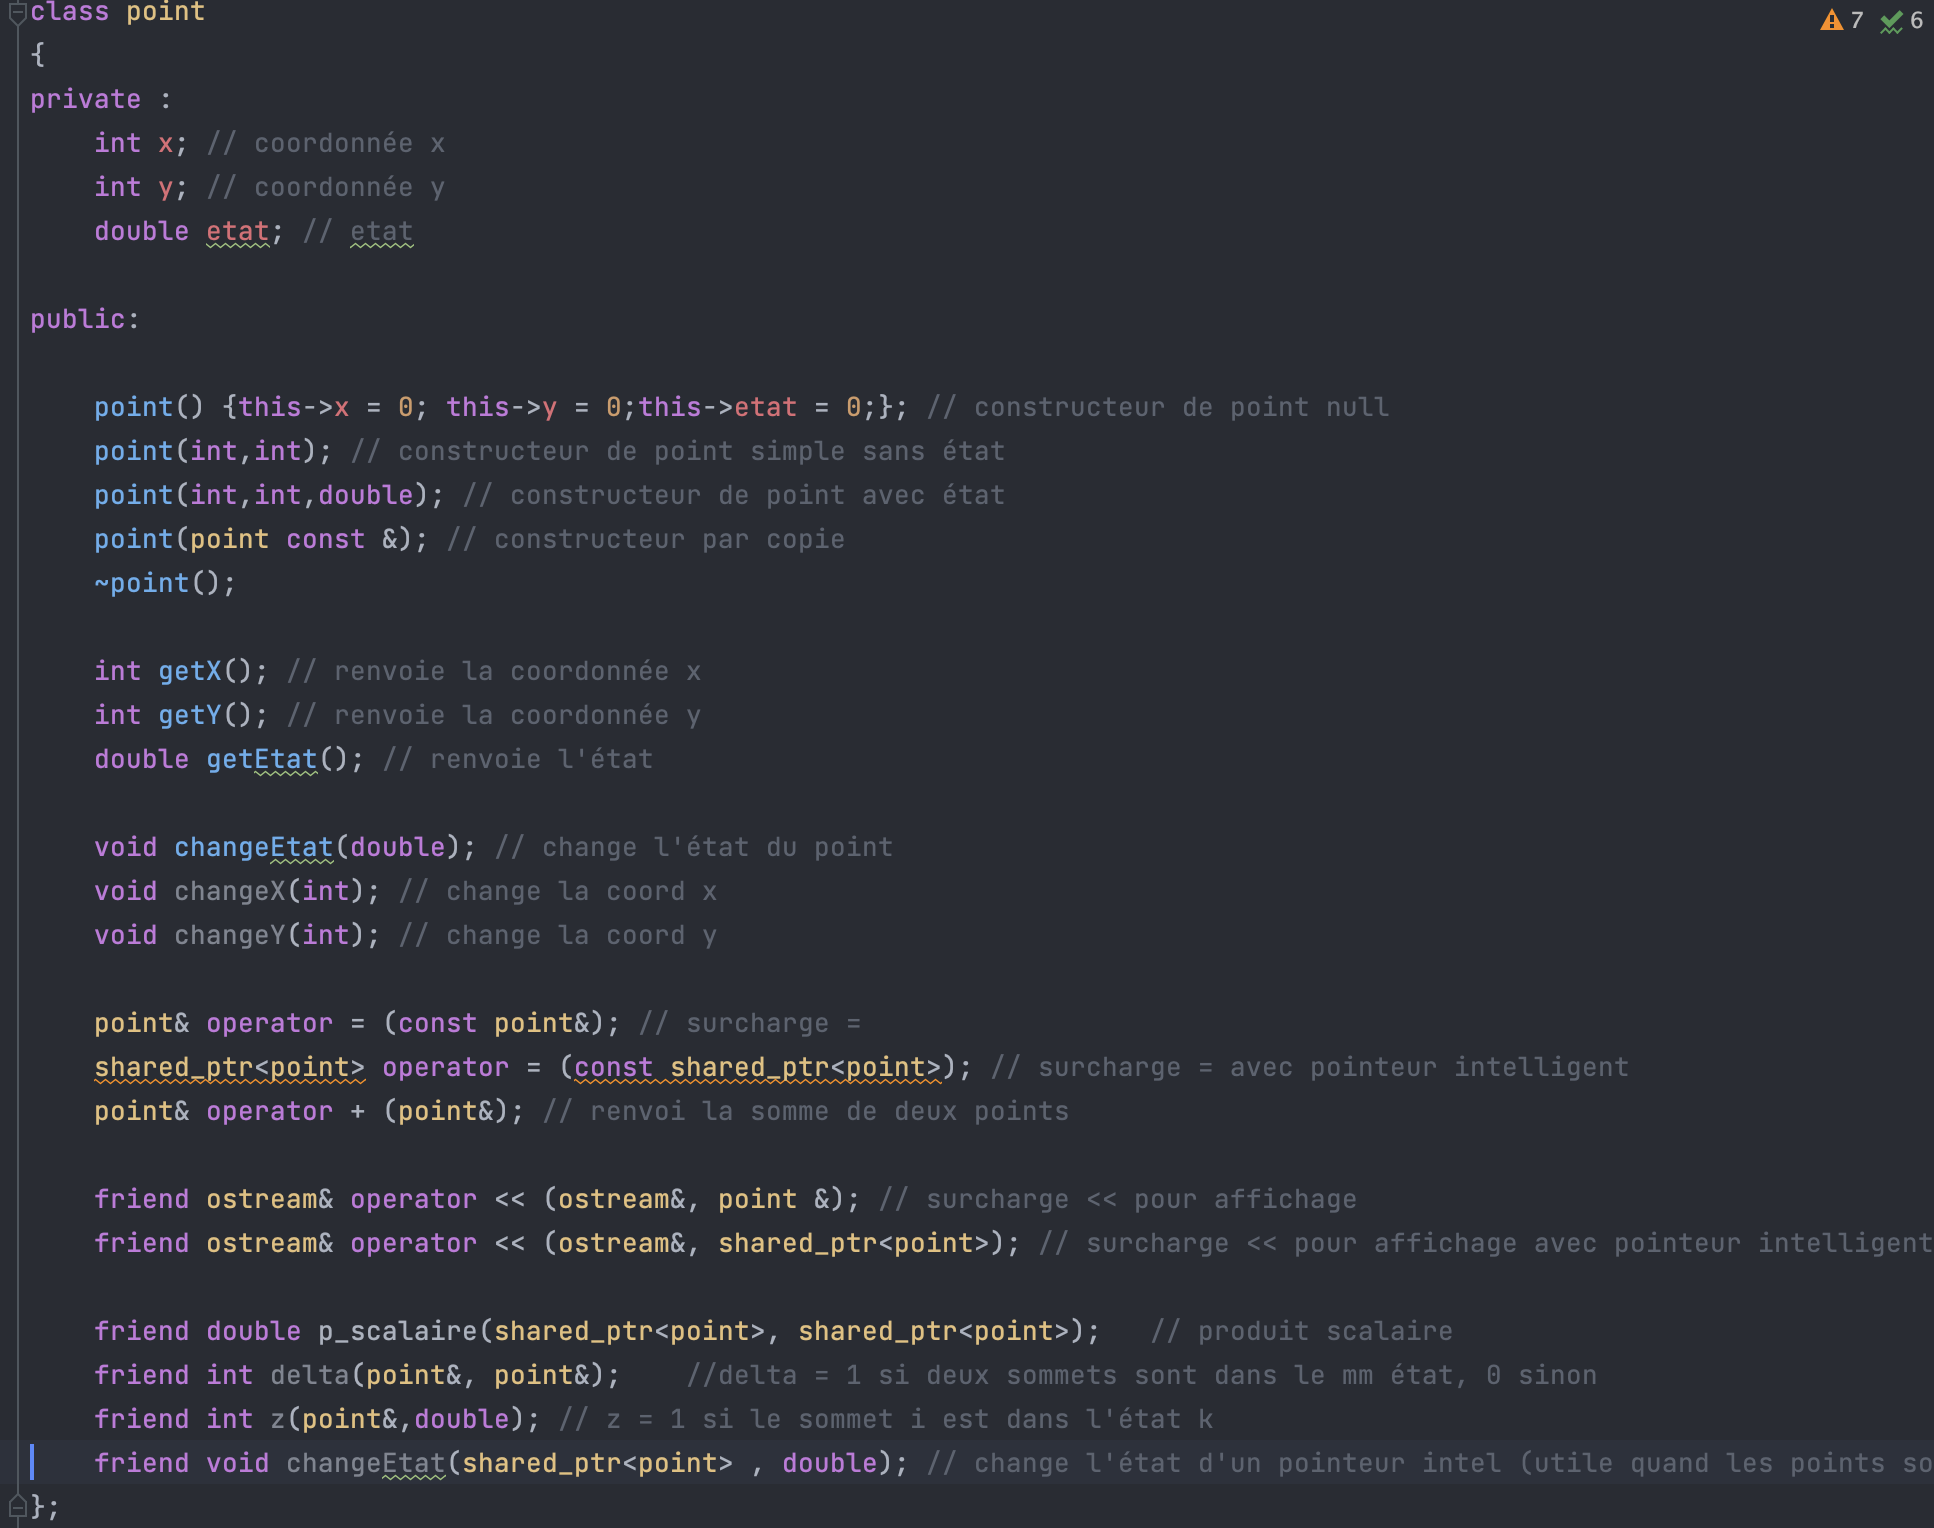
\includegraphics[width=0.9\textwidth, inner]{./img/prog/point/fichier_header_point}
        \caption{Header de la classe Point}
        \label{fig:prog2}
    \end{figure}
    ddzdz
\end{article} %explication de la partie prog

\chapter*{Théorie}
\addcontentsline{toc}{chapter}{Théorie}
\newcommand\tab[1][0.8cm]{\hspace*{#1}}

% Document
\section{Clustering}
\addcontentsline{toc}{section}{Clustering}

\begin{article}

Le principe du clustering est d'identifier des groupes(cluster) dans un jeu de données et de classer les observations
de ce jeu de données dans ces groupes selon des critères que nous verrons par la suite.
\newline L'algorithme de clustering le plus répandu est celui des K-means (K-moyennes). Soit $x_i \in \mathbb{R}^d,
i = 1,\dots,n,$ on souhaite répartir ces n points en q clusters. Soit $z_{ki} = 1$ si $x_i$ appartient au k-ème cluster, 0
sinon.
\newline
\newline L'algorithme des K-moyennes consiste à:
\newline
\newline (i) Trouver les centres des clusters que l'on note $\{m_k\}_{k=1}^{q}$ ainsi que les membres $z_{ki}$ de ces
clusters. Ces membres sont obetnus en minimisant la quantité $\frac{1}{n}\sum_{k=1}^{q}\sum_{i=1}^{n}z_{ki}(x_i-m_k)^t(x_i-m_k)$
ce qui revient à maximiser $\frac{1}{n}\sum_{i=1}^{n}\sum_{j=1}^{n}\langle x_i,x_j \rangle\sum_{k=1}^{q}\frac{z_{ki}z_{kj}}{n_k} $
où $n_k$ est le nombre de points du k-ème cluster, $k=1,\dots,q$ et $\langle \cdot,\cdot \rangle$ le produit scalaire sur $\mathbb{R}^d$.
\newline
\newline (ii) Les poids $w(i,j,\{z_{ki}\})$ qui sont égales à $\frac{1}{n_k}$ si $x_i$ et $x_j$ sont dans le même cluster k,
zéro sinon.



\end{article} %explication algorithme metropolis hasting

\end{document} 